\documentclass[twocolumn, natbib]{svjour3}
%DIF LATEXDIFF DIFFERENCE FILE
%DIF DEL revision/report/report.tex    Mon Mar 23 13:09:48 2015
%DIF ADD revision2/report/report.tex   Sat Apr 18 02:33:00 2015
\usepackage{graphicx}%GRaphiken
\usepackage[utf8]{inputenc}
\usepackage{tabularx}%Tabellen!
\usepackage[english]{babel}
\usepackage{textcomp}% Sonderzeichen
\usepackage{amsmath}%maths / equations
\usepackage{mathptmx}
\usepackage{url}
\usepackage{marvosym}
%DIF 11a11
\usepackage{todonotes} %DIF > 
%DIF -------
\newcommand{\envelope}{(\raisebox{-.5pt}{\scalebox{1.45}{\Letter}}\kern-.1pt) }

% to compare to old
% cd /home/edisz/Documents/Uni/Projects/PHD/6USETHEGLM/manuscript/
%DIF 15-16d16
%DIF < % % first compare bibliography
%DIF < % latexdiff submission/report/report.bbl revision/report/report.bbl > revision/diff/diff.bbl
%DIF -------

% % then document
%DIF 19c18
%DIF < % latexdiff --disable-citation-markup --math-markup=3 --append-context2cmd=subtitle submission/report/report.tex revision/report/report.tex > revision/diff/diff.tex
%DIF -------
% latexdiff --disable-citation-markup --math-markup=3 --append-context2cmd=subtitle revision/report/report.tex  revision2/report/report.tex > revision2/diff/diff.tex %DIF > 
%DIF -------



%% ----------------------------------------------------------------------------
\title{Ecotoxicology is not normal.}
\subtitle{A comparison of statistical approaches for analysis of count and proportion data in ecotoxicology.}
\author{Eduard Szöcs \and Ralf B. Schäfer}
\institute{Eduard Szöcs \envelope  and Ralf B. Schäfer \at
Institute for Environmental Sciences \\
University Koblenz-Landau \\
Fortstraße 7, \\
76829 Landau, Germany \\
Tel.: +49 06341 280 31552 \\
\email{szoecs@uni-landau.de}
}
\date{Received: date / Accepted: date}
\journalname{Environmental Science and Pollution Research}



%% ----------------------------------------------------------------------------
%DIF PREAMBLE EXTENSION ADDED BY LATEXDIFF
%DIF UNDERLINE PREAMBLE %DIF PREAMBLE
\RequirePackage[normalem]{ulem} %DIF PREAMBLE
\RequirePackage{color}\definecolor{RED}{rgb}{1,0,0}\definecolor{BLUE}{rgb}{0,0,1} %DIF PREAMBLE
\providecommand{\DIFadd}[1]{{\protect\color{blue}\uwave{#1}}} %DIF PREAMBLE
\providecommand{\DIFdel}[1]{{\protect\color{red}\sout{#1}}}                      %DIF PREAMBLE
%DIF SAFE PREAMBLE %DIF PREAMBLE
\providecommand{\DIFaddbegin}{} %DIF PREAMBLE
\providecommand{\DIFaddend}{} %DIF PREAMBLE
\providecommand{\DIFdelbegin}{} %DIF PREAMBLE
\providecommand{\DIFdelend}{} %DIF PREAMBLE
%DIF FLOATSAFE PREAMBLE %DIF PREAMBLE
\providecommand{\DIFaddFL}[1]{\DIFadd{#1}} %DIF PREAMBLE
\providecommand{\DIFdelFL}[1]{\DIFdel{#1}} %DIF PREAMBLE
\providecommand{\DIFaddbeginFL}{} %DIF PREAMBLE
\providecommand{\DIFaddendFL}{} %DIF PREAMBLE
\providecommand{\DIFdelbeginFL}{} %DIF PREAMBLE
\providecommand{\DIFdelendFL}{} %DIF PREAMBLE
%DIF END PREAMBLE EXTENSION ADDED BY LATEXDIFF

\begin{document}
\sloppy
\maketitle

%% ----------------------------------------------------------------------------
\begin{abstract}
Counts and proportions are data types often encountered by ecotoxicologists, which are rarely normally distributed.
To meet the assumptions of \DIFdelbegin \DIFdel{normality and heteroscedasticity, the standard procedure has been to either transform the data or use }\DIFdelend \DIFaddbegin \DIFadd{the linear model such data are often transformed or }\DIFaddend non-parametric methods \DIFaddbegin \DIFadd{used }\DIFaddend if this fails.
Generalised Linear Models (GLM) allow directly model \DIFdelbegin \DIFdel{distributions fitting such data}\DIFdelend \DIFaddbegin \DIFadd{such data, without the need for transformation}\DIFaddend .
Here, we compare the performance of parametric methods assuming (1) normality of transformed data, (2) appropriate distributions (Poisson, negativ binomial, binomial) and (3) non-parametric methods.

We simulated typical data mimicking low replicated ecotoxicological experiments of two common data types (counts and proportions from counts). 
We compared the performance of \DIFaddbegin \DIFadd{the }\DIFaddend different methods in terms of statistical power and \DIFdelbegin \DIFdel{type 1 }\DIFdelend \DIFaddbegin \DIFadd{Type I }\DIFaddend error for detecting a general treatment effect and determining the lowest observed effect concentration (LOEC).
In addition, we outlined differences \DIFdelbegin \DIFdel{and advantages of GLMs }\DIFdelend on a real world mesocosm data set.

For \DIFdelbegin \DIFdel{counts}\DIFdelend \DIFaddbegin \DIFadd{count data}\DIFaddend , we found that the quasi-Poisson model \DIFdelbegin \DIFdel{and the }\DIFdelend \DIFaddbegin \DIFadd{yielded highest power. The }\DIFaddend negative binomial model \DIFdelbegin \DIFdel{in combination with the parametric boostrap had higher statistical power than data transformation}\DIFdelend \DIFaddbegin \DIFadd{resulted in increased Type I errors , which could be fixed using the parametric bootstrap}\DIFaddend . 
For proportions\DIFaddbegin \DIFadd{, binomial }\DIFaddend GLMs performed better \DIFaddbegin \DIFadd{than assuming normality of transformed data}\DIFaddend , except to determine LOEC at \DIFdelbegin \DIFdel{extremly }\DIFdelend \DIFaddbegin \DIFadd{extremely }\DIFaddend low sample sizes.
The compared non-parametric methods had generally lower power.

We recommend that counts \DIFaddbegin \DIFadd{in one factorial experiments should be analysed using quasi-Poisson models }\DIFaddend and proportions from counts \DIFdelbegin \DIFdel{should be analysed by making appropriate distributional assumptions and GLMsshould become a standard method }\DIFdelend \DIFaddbegin \DIFadd{by binomial GLMs.
These methods should become standard }\DIFaddend in ecotoxicology.
 \DIFdelbegin %DIFDELCMD < \keywords{Generalized Linear Models \and Transformations \and Simulation \and Power \and Type 1 error}
%DIFDELCMD < %%%
\DIFdelend \DIFaddbegin \keywords{Generalized Linear Models \and Transformations \and Simulation \and Power \and Type I error}
\DIFaddend \end{abstract}



%% ----------------------------------------------------------------------------
\section{Introduction}
\label{sec:intro}
Ecotoxicologists perform various kinds of experiments yielding different types of data.
Examples are animal counts in mesocosm experiments (non-negative, integer-valued data) or proportions of surviving animals (data bounded between 0 and 1, discrete).
These data are typically not normally distributed. 
Nevertheless, \DIFdelbegin \DIFdel{they }\DIFdelend \DIFaddbegin \DIFadd{such data }\DIFaddend are often analysed using methods \DIFdelbegin \DIFdel{assuming }\DIFdelend \DIFaddbegin \DIFadd{that assume }\DIFaddend a normal distribution and variance homogeneity \citep{wang_making_2011}. 
To meet these assumptions \DIFdelbegin \DIFdel{, }\DIFdelend data are usually transformed.
For example, ecotoxicological textbooks \citep{newman_quantitative_2012} and guidelines \citep{epa_methods_2002,oecd_current_2006} advise that survival data \DIFdelbegin \DIFdel{can }\DIFdelend \DIFaddbegin \DIFadd{should }\DIFaddend be transformed using an arcsine square root transformation. 
For count data from mesocosm experiments a log(Ay + C) transformation is usually applied, where the constants A and C are either chosen arbitrarily or following general recommendations. 
For example, \citet{van_den_brink_impact_2000} suggest to set the term Ay to be 2 for the lowest abundance value (y) greater than zero and C to 1. 
\DIFdelbegin \DIFdel{Moreover, other transformations}\DIFdelend \DIFaddbegin \DIFadd{Other transformations, }\DIFaddend like the square root or fourth root \DIFdelbegin \DIFdel{are }\DIFdelend \DIFaddbegin \DIFadd{transformation, are also }\DIFaddend commonly applied in community ecology \DIFaddbegin \citep{anderson_navigating_2011}\DIFaddend .
Note that there has been little evaluation and advice for practitioners \DIFdelbegin \DIFdel{, }\DIFdelend which transformations to use.
If the transformed data still do not meet the assumptions \DIFdelbegin \DIFdel{(i.e. normality and variance homogeneity)}\DIFdelend \DIFaddbegin \DIFadd{of the linear model}\DIFaddend , non-parametric tests are usually applied \citep{wang_making_2011}.

Generalised linear models (GLM) provide a method to analyse counts or proportions from counts in a  statistically sound way \citep{nelder_generalized_1972}.
GLMs can handle various types of data distributions, e.g. Poisson or negative binomial (for count data) or binomial (for proportions); the normal distribution being a special case of GLMs.
Despite GLMs being available \DIFaddbegin \DIFadd{for }\DIFaddend more than 40 years, ecotoxicologists do not regularly make use of them.
Recent studies concluded that \DIFdelbegin \DIFdel{data transformations should be avoided }\DIFdelend \DIFaddbegin \DIFadd{the linear model should not be applied on transformed data }\DIFaddend and GLMs be used as they have better statistical properties (\DIFdelbegin %DIFDELCMD < \citealt{ohara_not_2010} %%%
\DIFdelend \DIFaddbegin \citealt{ohara_not_2010,warton_many_2005} \DIFaddend (counts), \DIFdelbegin %DIFDELCMD < \citealt{warton_arcsine_2011,warton_many_2005} %%%
\DIFdelend \DIFaddbegin \citealt{warton_arcsine_2011} \DIFaddend (proportions from counts)). 

Ecotoxicological experiments often involve small sample sizes due to practical constraints. 
For example, extremely low samples sizes (n \textless 5) are common in many mesocosm studies \citep{sanderson_pesticide_2002,szocs_analysing_2015}.
Small sample sizes lead to low power in statistical hypothesis testing, on which many ecotoxiological approaches (e.g. risk assessment for pesticides) rely. 
Such an endpoint are L/NOEC \DIFaddbegin \DIFadd{values }\DIFaddend (Lowest / No observed effect concentration)\DIFdelbegin \DIFdel{values}\DIFdelend .
Although their use has been heavily criticized in the past \citep{laskowski_good_1995}, they are the predominant endpoint in mesocosm experiments \citep{brock_minimum_2015, efsa_ppr_guidance_2013}. 

We explore how GLMs may enhance\DIFaddbegin \DIFadd{, when appropriately used, }\DIFaddend inference in ecotoxicological studies and compared three types of statistical methods (\DIFdelbegin \DIFdel{transformation and normality assumption}\DIFdelend \DIFaddbegin \DIFadd{linear model on transformed data}\DIFaddend , GLM, non-parametric tests).
We first illustrate differences between statistical methods using a data set from a mesocosm study.
Then we further elaborate differences in detecting a general treatment effect and determining the LOEC using simulations of two common data types in ecotoxicology: counts and proportions from counts. 



%% ----------------------------------------------------------------------------
\section{Methods}
\label{sec:methods}

%% --------------------------------
\subsection{Models for count data}
\label{ssec:counts}
\subsubsection{Linear model for transformed data}
To meet the assumptions of the standard linear model, count data usually needs to be transformed. 
We followed the recommendations of \citet{van_den_brink_impact_2000} and used a log(Ay + 1) transformation (eqn. \ref{eqn:trans}):
\begin{align}
  \DIFdelbegin \DIFdel{y_i^T }\DIFdelend \DIFaddbegin \DIFadd{Y_{new~i} }\DIFaddend & = log(\DIFdelbegin \DIFdel{Ay}\DIFdelend \DIFaddbegin \DIFadd{AY}\DIFaddend _i + 1) \label{eqn:trans}
\end{align}

, where \DIFdelbegin \DIFdel{$y_i$ }\DIFdelend \DIFaddbegin \DIFadd{$Y_i$ }\DIFaddend is the measured and \DIFdelbegin \DIFdel{$y_i^T$ }\DIFdelend \DIFaddbegin \DIFadd{$Y_{new~i}$ }\DIFaddend the transformed abundance of the $i$th observation. 
The factor $A$ was chosen in such way that \DIFdelbegin \DIFdel{$Ay$ }\DIFdelend \DIFaddbegin \DIFadd{$AY$ }\DIFaddend equals 2 for the lowest non-zero abundance value (\DIFdelbegin \DIFdel{y}\DIFdelend \DIFaddbegin \DIFadd{Y}\DIFaddend ).

Then we fitted the linear model to the transformed abundances (hereafter $LM$):
\begin{align}
  \DIFdelbegin \DIFdel{y_i^T }\DIFdelend \DIFaddbegin \DIFadd{Y_{new~i} }\DIFaddend &\sim N(\mu_i, \sigma^2) \nonumber \\
  E(\DIFdelbegin \DIFdel{y_i^T}\DIFdelend \DIFaddbegin \DIFadd{Y_{new~i}}\DIFaddend ) = \mu_i ~&\text{and}~ var(\DIFdelbegin \DIFdel{y_i^T}\DIFdelend \DIFaddbegin \DIFadd{Y_{new~i}}\DIFaddend ) = \sigma^2 \label{eqn:normal} \\
  \mu_i &= \beta \DIFdelbegin \DIFdel{Treatment}\DIFdelend \DIFaddbegin \DIFadd{\times X}\DIFaddend _i  \nonumber
\end{align}

This model assumes a normal distribution of the transformed abundances.
The expected value for each observation $i$ is given by its mean ($\mu_i$) and the variance ($\sigma^2$) is constant between treatments.
We allow this mean to vary between treatments \DIFaddbegin \DIFadd{($X_i$ codes the treatments) }\DIFaddend and $\beta$ are the \DIFaddbegin \DIFadd{estimated }\DIFaddend coefficients related to these changes in transformed abundances between treatments (eqn. \ref{eqn:normal}).


\subsubsection{Generalised Linear Models}
GLMs extend the \DIFdelbegin \DIFdel{normal model by modelling other distributions}\DIFdelend \DIFaddbegin \DIFadd{linear model to variables that are not normally distributed}\DIFaddend .
Instead of transforming the response variable, the counts could be directly modelled by a Poisson GLM ($GLM_p$):
\begin{align}
  \DIFdelbegin \DIFdel{y}\DIFdelend \DIFaddbegin \DIFadd{Y}\DIFaddend _i &\sim P(\mu_i) \nonumber \\
  E(\DIFdelbegin \DIFdel{y}\DIFdelend \DIFaddbegin \DIFadd{Y}\DIFaddend _i) &= var(\DIFdelbegin \DIFdel{y}\DIFdelend \DIFaddbegin \DIFadd{Y}\DIFaddend _i) = \mu_i \label{eqn:pois} \\
  log(\mu_i) &= \beta \DIFdelbegin \DIFdel{Treatment}\DIFdelend \DIFaddbegin \DIFadd{\times X}\DIFaddend _i  \nonumber
\end{align}

This model assumes \DIFdelbegin \DIFdel{poisson }\DIFdelend \DIFaddbegin \DIFadd{Poisson }\DIFaddend distributed abundances with mean $\mu_i \ge 0$.
The expected value for each observation $i$ is given by its mean. 
Moreover, this model assumes that mean and variance are equal.
We are modelling the mean as a function of treatment membership \DIFaddbegin \DIFadd{($X_i$)}\DIFaddend .
However, to avoid negative values of the mean this is done on a log scale.
Therefore, $\beta$ also describes the differences between treatments on a log scale (eqn. \ref{eqn:pois}).

The assumption of equal mean and variance is rarely met with ecological data, which is typically characterized by greater variance than the mean (overdispersion).
To overcome this problem a quasi-Poisson model ($GLM_{qp}$) could be used, which \DIFdelbegin \DIFdel{assumes that variance is }\DIFdelend \DIFaddbegin \DIFadd{models the variance as }\DIFaddend a linear function of the mean (eqn. \ref{eqn:quasi}):
\begin{align}
  var(\DIFdelbegin \DIFdel{y}\DIFdelend \DIFaddbegin \DIFadd{Y}\DIFaddend _i) &= \DIFdelbegin \DIFdel{\Theta }\DIFdelend \DIFaddbegin \DIFadd{\phi }\DIFaddend \mu_i  \label{eqn:quasi}
\end{align}

Here, \DIFdelbegin \DIFdel{$\Theta$ }\DIFdelend \DIFaddbegin \DIFadd{$\phi$ }\DIFaddend is used to account for additional variation and is known as overdispersion parameter.
The quasi-Poisson model is a post hoc method, meaning that first a Poisson model is estimated (eqn. \ref{eqn:pois}) and than the standard errors are scaled by the degree of overdispersion \DIFaddbegin \citep{hilbe_modeling_2014}\DIFaddend .

Another possibility to deal with overdispersion is to \DIFdelbegin \DIFdel{fit }\DIFdelend \DIFaddbegin \DIFadd{model abundances by }\DIFaddend a negative binomial distribution ($GLM_{nb}$, eqn. \ref{eqn:negbin}):
\begin{align}
  \DIFdelbegin \DIFdel{y}\DIFdelend \DIFaddbegin \DIFadd{Y}\DIFaddend _i &\sim NB(\mu_i, \kappa) \nonumber  \\
  E(\DIFdelbegin \DIFdel{y}\DIFdelend \DIFaddbegin \DIFadd{Y}\DIFaddend _i) = \mu_i ~&\text{and}~var(\DIFdelbegin \DIFdel{y}\DIFdelend \DIFaddbegin \DIFadd{Y}\DIFaddend _i) = \mu_i + \mu_i^2 / \kappa \label{eqn:negbin} \\
  log(\mu_i) &= \beta \DIFdelbegin \DIFdel{Treatment}\DIFdelend \DIFaddbegin \DIFadd{\times X}\DIFaddend _i  \nonumber 
\end{align}

This models assumes that abundances are negative binomially distributed, with a mean of $\mu_i \ge 0$ and a variance $\mu_i + \mu_i^2 / \kappa$.
Similar to the Poisson model we use a log link between mean and treatments.
Note, that the quasi-Poisson model assumes a linear mean-variance relationship (eqn. \ref{eqn:quasi}), whereas the negative binomial model assumes a quadratic relationship (eqn. \ref{eqn:negbin}).

The above described models are most commonly used in ecology \citep{ver_hoef_quasi-poisson_2007}, although other distributions for count data are possible, like the negative binomial model with a linear mean-variance relationship (also known as NB1) or the poisson inverse gaussian model \citep{hilbe_modeling_2014}.


\subsection{Models for binomial data}
\label{ssec:bin}
A binomial variable counts how often an event $x$ occurs in a fixed number of independent trials $N$ (e.g. \emph{"5 out of 10 fish survived"}), with an equal probability of occurrence $\pi$ between trials.
The number of times an event occurs can also be calculated as proportion $x / N$.

\subsubsection{Linear model for transformed data}
To accommodate the assumptions for the standard linear model with such proportions, a special arcsine square root transformation (eqn. \ref{eqn:arcsine}) is suggested \citep{epa_methods_2002,newman_quantitative_2012}:
\begin{align}
  \DIFdelbegin \DIFdel{y_i^T }\DIFdelend \DIFaddbegin \DIFadd{Y_{new~i} }\DIFaddend = 
  \begin{cases}  
    arcsin(1) - arcsin(\sqrt{\frac{1}{4n}}) & \text{, if}\ \DIFdelbegin \DIFdel{y}\DIFdelend \DIFaddbegin \DIFadd{Y}\DIFaddend _i = 1 \\
    arcsin(\sqrt{\frac{1}{4n}}) & \text{, if}\ \DIFdelbegin \DIFdel{y}\DIFdelend \DIFaddbegin \DIFadd{Y}\DIFaddend _i = 0  \\
    arcsin(\sqrt{\DIFdelbegin \DIFdel{y}\DIFdelend \DIFaddbegin \DIFadd{Y}\DIFaddend _i}) & \text{, otherwise}
  \end{cases} \label{eqn:arcsine}
\end{align}

, where \DIFdelbegin \DIFdel{$y_i^T$ are the }\DIFdelend \DIFaddbegin \DIFadd{$Y_i$ are the untransformed proportions, $Y_{new~i}$ are the }\DIFaddend transformed proportions and n is the total number of exposed animals per treatment.
The transformed proportions are then analysed using the standard linear model ($LM$, eqn. \ref{eqn:normal}).
Note, that the \DIFdelbegin \DIFdel{parameters }\DIFdelend \DIFaddbegin \DIFadd{coefficients }\DIFaddend of the linear model are not directly interpretable due to transformation.


\subsubsection{Generalised Linear Models}
A more natural way to model such data is the  binomial distribution with parameters N and $\pi$ ($GLM_{bin})$:
\begin{align}
  \DIFdelbegin \DIFdel{y}\DIFdelend \DIFaddbegin \DIFadd{Y}\DIFaddend _i &\sim Bin(N, \pi_i) \nonumber \\
  E(\DIFdelbegin \DIFdel{y}\DIFdelend \DIFaddbegin \DIFadd{Y}\DIFaddend _i) = \pi_i \times N ~&\text{and}~var(\DIFdelbegin \DIFdel{y}\DIFdelend \DIFaddbegin \DIFadd{Y}\DIFaddend _i) =  \pi_i (1 - \pi_i) / N \label{eqn:bin} \\
  logit~(\pi_i) &= \beta \DIFdelbegin \DIFdel{Treatment}\DIFdelend \DIFaddbegin \DIFadd{\times X}\DIFaddend _i \nonumber
  \end{align}

This model assumes that the number of \DIFdelbegin \DIFdel{occurences }\DIFdelend \DIFaddbegin \DIFadd{occurrences ($Y_i$) }\DIFaddend are binomially distributed, where N = number of trials (e.g. exposed animals) and $\pi_i$ is the probability of occurrences (fish survived), which together give the expected number of occurrences.
The variance of the binomial distribution is a quadratic function of the mean.
We are modelling the probability of occurrence as function of treatment membership \DIFaddbegin \DIFadd{($X_i$) }\DIFaddend and to ensure that $0 < \pi_i < 1$ we do this on a logit scale (eqn. \ref{eqn:bin}). 
\DIFdelbegin \DIFdel{However, the parameters }\DIFdelend \DIFaddbegin \DIFadd{The estimated coefficients (}\DIFaddend $\beta$\DIFaddbegin \DIFadd{) }\DIFaddend of this model are directly interpretable as changes in log odds between treatments.

\DIFdelbegin \DIFdel{Similarly to counts, binomial data may also show overdispersion }\DIFdelend \DIFaddbegin \DIFadd{Non-independent trials (e.g. fish are grouped in aquaria) may lead to overdispersion }\citep{williams_extra-binomial_1982}\DIFaddend .
Methods to deal with overdispersed binomial data are \DIFdelbegin \DIFdel{either }\DIFdelend \DIFaddbegin \DIFadd{for example }\DIFaddend quasi methods (see above) or Generalized Linear Mixed models (GLMM).
However, these are not further investigated in this paper (see \citet{warton_arcsine_2011} for a comparison).


%% --------------------------------
\subsection{Statistical Inference}
After model fitting \DIFdelbegin \DIFdel{and parameter estimation }\DIFdelend the next step is statistical inference.
Ecotoxicologists are generally interested in two hypotheses: (i) is there any treatment related effect? and (ii) which treatments show a treatment effect (to determine the LOEC)?

Following general recommendations \citep{bolker_generalized_2009,faraway_extending_2006}, we used F-tests ($LM$ and $GLM_{qp}$) and Likeli\-hood-Ratio (LR) tests ($GLM_p$, $GLM_{nb}$ and $GLM_{bin}$) to test the first hypothesis.
However, it is well known that \DIFdelbegin \DIFdel{LR test are }\DIFdelend \DIFaddbegin \DIFadd{the LR test is }\DIFaddend unreliable with small sample sizes \citep{wilks_large-sample_1938}.
Therefore, we additionally explored the parametric bootstrap \citep{faraway_extending_2006} to assess the significance of the LR.
Bootstrapping is computationally very intensive and for this reason we applied it only for the \DIFaddbegin \DIFadd{LR test of the }\DIFaddend negative binomial models (using 500 bootstrap samples, denoted as $GLM_{npb}$).

To assess the LOEC we used Dunnett contrasts \citep{dunnett_multiple_1955} with one-sided Wald t tests (normal and quasi-Poisson models) and one-sided Wald Z tests (Poisson, negative binomial and binomial models).
Beside these parametric methods we also applied two, in ecotoxicology commonly used, non-parametric methods: The Kruskal-Wallis test  ($KW$) to test for a general treatment effect and a pairwise Wilcoxon test ($WT$) to determine the LOEC.
We adjusted for multiple testing using the method of \citet{holm_simple_1979}.



%% --------------------------------
\subsection{Case study}
\citet{brock_minimum_2015} presents a typical example of data from mesocosm studies, which we use to demonstrate differences between methods.
The data are mayfly larvae counts on artificial substrate samplers \DIFdelbegin \DIFdel{were }\DIFdelend at one sampling date. 
A total of 18 \DIFdelbegin \DIFdel{mesocosm }\DIFdelend \DIFaddbegin \DIFadd{mesocosms }\DIFaddend have been sampled from 6 treatments (Control (n = 4), 0.1, 0.3, 1, 3 mg/L (n = 3) and 10 mg/L (n = 2)) (Figure \ref{fig:example}).

\begin{figure}[h]
  \centering
  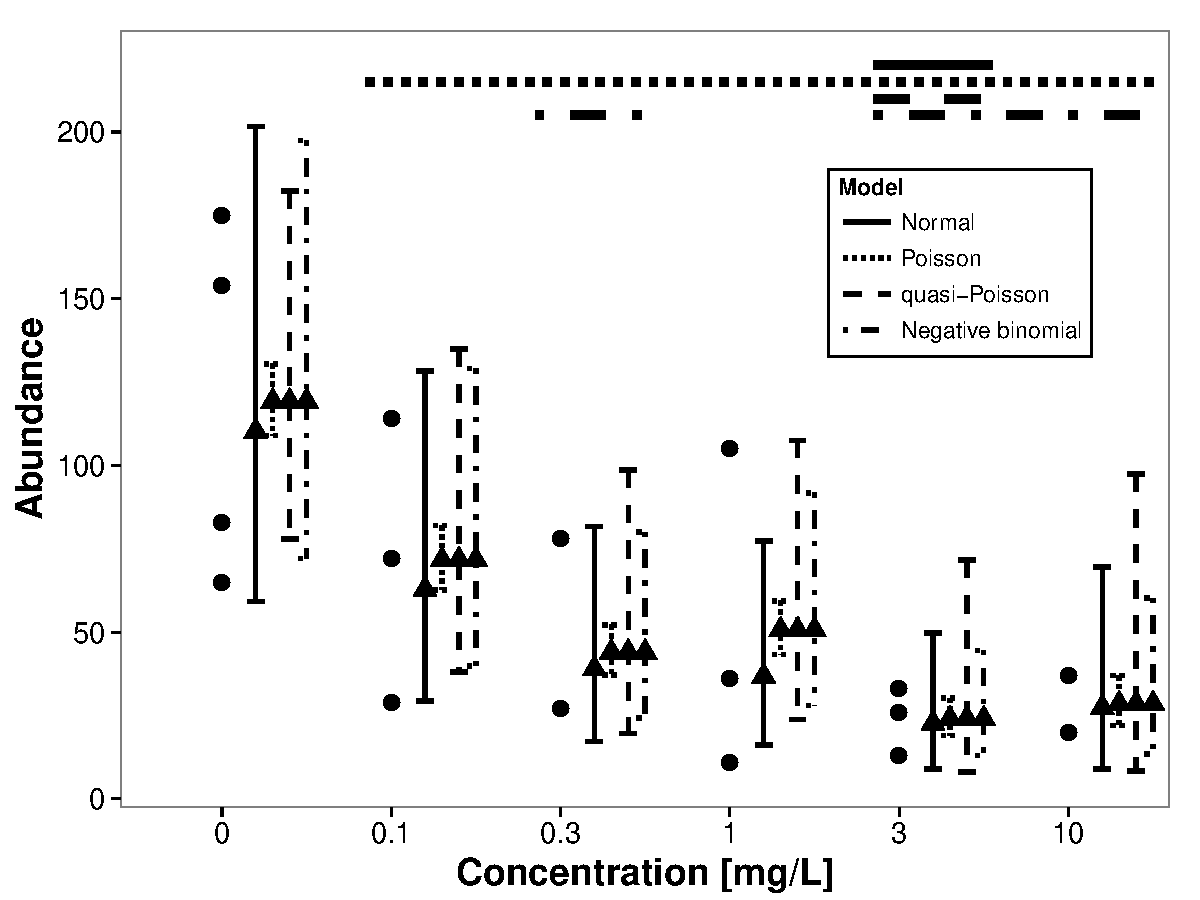
\includegraphics[width = 84mm]{example.pdf}
  \caption{Data from \citet{brock_minimum_2015} (dots). 
  Predicted values (triangles) and 95\% Wald Z or t confidence intervals from the fitted models (vertical lines) are given beside.
  Horizontal bars above indicate treatments statistically significant different from the control group (Dunnett contrasts).
  The data showed \DIFaddbeginFL \DIFaddFL{considerable }\DIFaddendFL overdispersion (\DIFdelbeginFL \DIFdelFL{$\kappa = 4$}\DIFdelendFL \DIFaddbeginFL \DIFaddFL{$\kappa = 3.91, \phi = 22.41$}\DIFaddendFL ) and therefore, the Poisson model underestimates the width of confidence intervals.
  }
  \label{fig:example}
\end{figure}


%% --------------------------------
\subsection{Simulations}
\subsubsection{Count data}
To further scrutinise the differences between methods we simulated data sets with known properties.
We simulated count data that mimics the data of the case study with five treatments (T1 - T5) and one control group (C).
Counts were drawn from a negative binomial distribution with overdispersion at all treatments ($\kappa = 4$, eqn. \ref{eqn:negbin}).
We simulated data sets with different number of replicates (N = \{3, 6, 9\}) and different abundances in control treatments ($\mu_\text{\tiny C}$ = \{2, 4, 8, 16, 32, 64, 128\}). 
For \DIFaddbegin \DIFadd{Type I error estimation mean abundance was equal between treatments.
For }\DIFaddend power estimation, mean abundance in treatments T2 - T5 was reduced to half of control and T1 ($\mu_\text{\tiny T2}~=~...~=~\mu_\text{\tiny T5}~=~0.5~\mu_\text{\tiny C} = 0.5~\mu_\text{\tiny T1}$), resulting in a theoretical LOEC at T2.
\DIFdelbegin \DIFdel{Mean abundance was kept equal between all groups in Type 1 error simulations.
}\DIFdelend We generated 1000 data sets for each combination of N and $\mu_\text{\tiny C}$ and analysed these using the models outlined in section \ref{ssec:counts}.


\subsubsection{Binomial data}
We simulated data from a commonly used design as described in \citet{weber_short-term_1989}, with 5 treated (T1 - T5) and \DIFdelbegin \DIFdel{a }\DIFdelend \DIFaddbegin \DIFadd{one }\DIFaddend control group (C). 
Proportions were drawn from a Bin(10, $\pi$) distribution, with varying probability of survival (\DIFdelbegin \DIFdel{$\pi_C$ }\DIFdelend \DIFaddbegin \DIFadd{$\pi$ }\DIFaddend = \{0.60, 0.65, 0.70, 0.75, 0.80, 0.85, 0.90, 0.95\}) and varying number of replicates (N = \{3, 6, 9\}).
For Type \DIFdelbegin \DIFdel{1 }\DIFdelend \DIFaddbegin \DIFadd{I }\DIFaddend error estimation, \DIFdelbegin \DIFdel{$\pi_C$ was held constant between groups}\DIFdelend \DIFaddbegin \DIFadd{$\pi$ was equal between treatments}\DIFaddend .
For power estimation \DIFdelbegin \DIFdel{$\pi_C$ in C and T1 }\DIFdelend \DIFaddbegin \DIFadd{$\pi$ }\DIFaddend was fixed at 0.95  \DIFdelbegin \DIFdel{and was set to values between 0.6 and 0.95 for the }\DIFdelend \DIFaddbegin \DIFadd{in C and T1 and varied only in }\DIFaddend treatments T2 - T5. 
For each combination we simulated 1000 data sets and analysed these using the models outlined in section \ref{ssec:bin}.

\subsection{Data Analysis}
We analysed the case study and the simulated data using the outlined methods.
We compared the methods and models in terms of Type \DIFdelbegin \DIFdel{1 }\DIFdelend \DIFaddbegin \DIFadd{I }\DIFaddend error (detection of an effect when there is none) and power (ability to detect an effect when it is present) \DIFaddbegin \DIFadd{at a significance level of $\alpha = 0.05$}\DIFaddend .

All simulations were done in R (Version 3.1.2) \citep{r_core_team_r:_2014} on an Amazon EC2 virtual Linux server (64bit, 15GB RAM, 8 cores, 2.8 GHz).
Source code to reproduce the simulations and paper is available online at \url{https://github.com/EDiLD/usetheglm}.
Moreover, Supplement 2 provides worked examples of the data of \citet{brock_minimum_2015} and \citet{weber_short-term_1989}.



%% ----------------------------------------------------------------------------
\section{Results}
\label{sec:results}
%% --------------------------------
\subsection{Case study}
The data set showed \DIFdelbegin \DIFdel{considerable }\DIFdelend \DIFaddbegin \DIFadd{considerably }\DIFaddend higher variance then expected by the Poisson model (\DIFdelbegin \DIFdel{$\Theta = 22.41$, }\DIFdelend \DIFaddbegin \DIFadd{$\phi = 22.41$ (}\DIFaddend eqn. \ref{eqn:quasi})\DIFdelbegin \DIFdel{. 
}\DIFdelend \DIFaddbegin \DIFadd{, $\kappa = 3.91$ (eqn. \ref{eqn:negbin})). 
}\DIFaddend Therefore, the Poisson model did not fit to this data and \DIFdelbegin \DIFdel{lead }\DIFdelend \DIFaddbegin \DIFadd{led }\DIFaddend to underestimated standard errors and confidence intervals, as well as overestimated statistical significance (Figure \ref{fig:example}).
In this case, inferences on the Poisson model are not valid and we do not further discuss its results.
The normal (F = 2.57, p = 0.084) and quasi-Poisson model (F = 2.90, p = 0.061), as well as the Kruskal test (p =  0.145) did not show a statistically significant treatment effects.
By contrast, the LR test and parametric bootstrap of the negative binomial model indicated a treatment-related effect (LR = 13.99, p = 0.016, bootstrap: p = 0.042).

All methods predicted similar values, except the normal model predicting always lower abundances (Figure \ref{fig:example}). 
95\%\DIFaddbegin \DIFadd{~}\DIFaddend confidence intervals (CI) where most narrow for the negative binomial model and widest for the quasi-Poisson model - especially at lower estimated abundances.
Consequently, the LOECs differed (Normal and quasi-Poisson: 3 mg/L, negative binomial: 0.3 mg/L).
The pairwise Wilcoxon test did not detect any treatment different from control.


%% --------------------------------
\subsection{Simulations}
\subsubsection{Count data}
For detecting a general treatment effect, $GLM_{nb}$ and $GLM_{p}$ showed inflated \DIFdelbegin \DIFdel{type 1 }\DIFdelend \DIFaddbegin \DIFadd{Type I }\DIFaddend error rates, whereas $KW$ was conservative at low sample sizes.
However, using \DIFaddbegin \DIFadd{the }\DIFaddend parametric bootstrap for the negative binomial model ($GLM_{npb}$)\DIFaddbegin \DIFadd{, as well as $LM$ and $GLM_{qp}$ }\DIFaddend resulted in appropriate \DIFdelbegin \DIFdel{type 1 }\DIFdelend \DIFaddbegin \DIFadd{Type I }\DIFaddend error rates.
For detecting a treatment effect,\DIFdelbegin \DIFdel{$GLM_{npb}$ and }\DIFdelend $GLM_{qp}$ \DIFdelbegin \DIFdel{exhibited higher powerthan }\DIFdelend \DIFaddbegin \DIFadd{had highest power, followed by $GLM_{npb}$, }\DIFaddend $LM$ and $KW$, the latter having least power (Figure \ref{fig:p_glob_c}).
For our simulation design (reduction in abundance by 50\%) a sample size per treatment of n = 9 was needed to achieve a power greater than 80\%.
At small sample sizes (n = {3, 6}) and low abundances ($\mu_C$ = {2, 4}) many of the negative binomial models ($GLM_{nb}$ and $GLM_{npb}$) did not converge to a solution (convergence rate \textless 85\% of the simulations, Supplement 1). 

\begin{figure*}
  \centering
  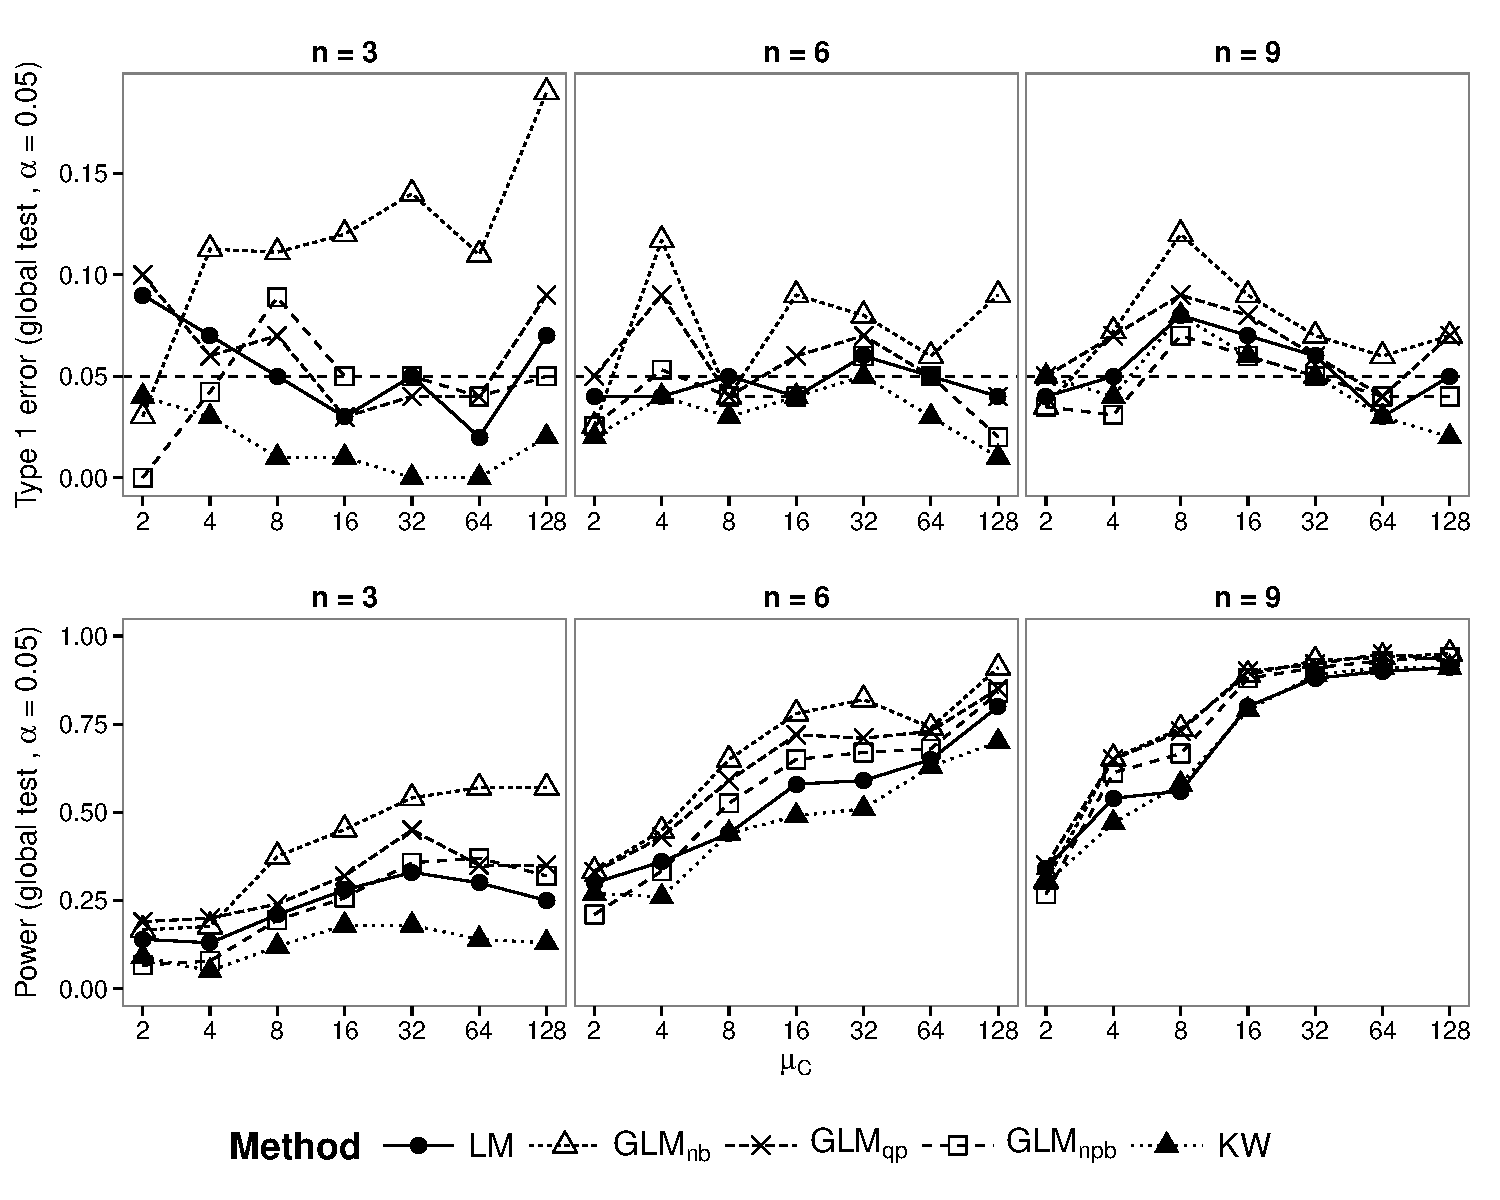
\includegraphics[width = 126mm]{p_glob_c.pdf}
  \caption{Count data simulations: Type \DIFdelbeginFL \DIFdelFL{1 }\DIFdelendFL \DIFaddbeginFL \DIFaddFL{I }\DIFaddendFL error (top) and Power (bottom) for the test of a treatment effect.
  Only \DIFdelbeginFL \DIFdelFL{type 1 }\DIFdelendFL \DIFaddbeginFL \DIFaddFL{Type I }\DIFaddendFL errors \textless 25\% are displayed. 
  $GLM_p$ showed \DIFdelbeginFL \DIFdelFL{type 1 }\DIFdelendFL \DIFaddbeginFL \DIFaddFL{Type I }\DIFaddendFL errors \textgreater 20\% in all simulation scenarios.
  Power levels for models with inflated \DIFdelbeginFL \DIFdelFL{type }\DIFdelendFL \DIFaddbeginFL \DIFaddFL{Type }\DIFaddendFL I \DIFdelbeginFL \DIFdelFL{error }\DIFdelendFL \DIFaddbeginFL \DIFaddFL{errors ($GLM_P$ and $GLM_{qp}$) }\DIFaddendFL are shown for completeness.
  For n = \{3, 6\} and $\mu_C$ = \{2, 4\} less than 85\% of $GLM_{nb}$ and $GLM_{npb}$ models did converge.
  Dashed horizontal line denotes the nominal \DIFdelbeginFL \DIFdelFL{Type 1 }\DIFdelendFL \DIFaddbeginFL \DIFaddFL{I }\DIFaddendFL error rate at $\alpha = 0.05$.
  }
  \label{fig:p_glob_c}
\end{figure*}

For LOEC determination $GLM_{nb}$ and $GLM_{p}$ showed an increased Type \DIFdelbegin \DIFdel{1 }\DIFdelend \DIFaddbegin \DIFadd{I }\DIFaddend error and all other methods were slightly conservative.
The inferences on LOEC generally showed less power.
$LM$ showed a mean reduction of 20.7\% and $GLM_{qp}$ of 24.3 \%.
Power to detect the LOEC was highest for $GLM_{qp}$. 
$LM$ and $WT$ showed less power, with $WT$ having no power to detect the LOEC at low sample sizes (Figure \ref{fig:p_loec_c}).

\begin{figure*}
  \centering
  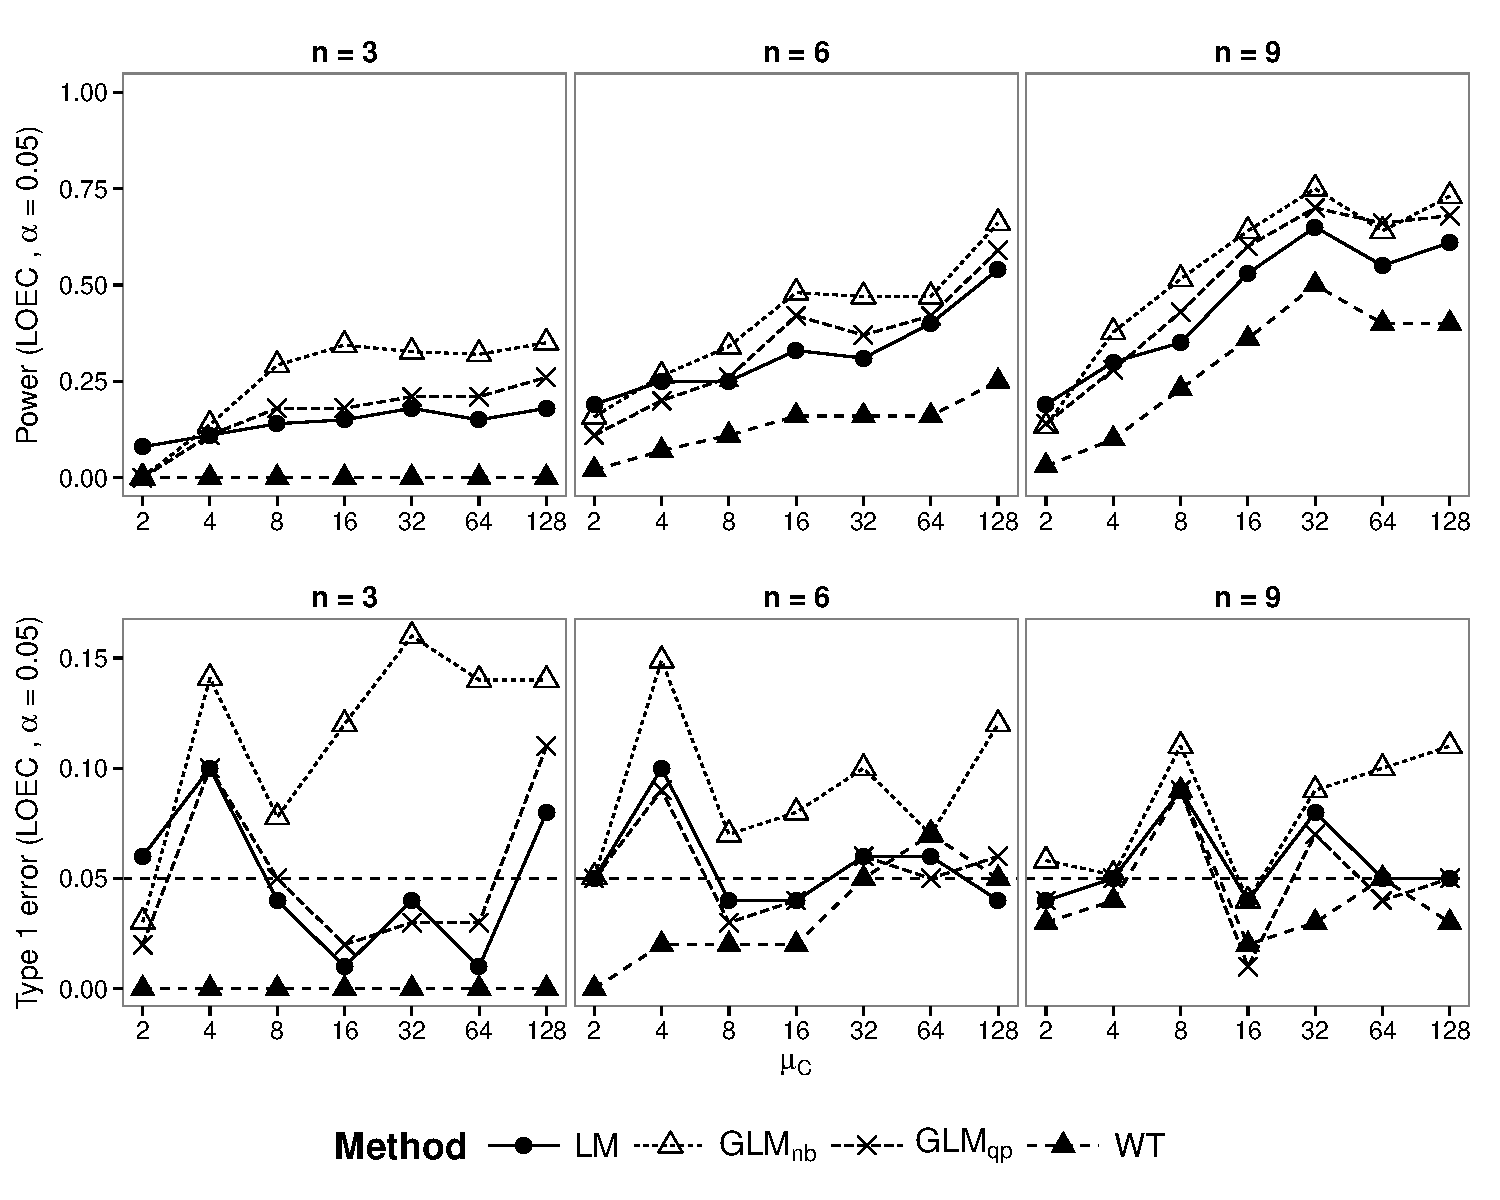
\includegraphics[width = 126mm]{p_loec_c.pdf}
  \caption{Count data simulations: Type \DIFdelbeginFL \DIFdelFL{1 }\DIFdelendFL \DIFaddbeginFL \DIFaddFL{I }\DIFaddendFL error (top) and Power (bottom) for determination of LOEC.
  For clarity only \DIFdelbeginFL \DIFdelFL{type 1 }\DIFdelendFL \DIFaddbeginFL \DIFaddFL{Type I }\DIFaddendFL errors \textless 25\% are displayed.
  Power levels for models with inflated \DIFdelbeginFL \DIFdelFL{type }\DIFdelendFL \DIFaddbeginFL \DIFaddFL{Type }\DIFaddendFL I error are shown for completeness.
  For n = \{3, 6\} and $\mu_C$ = \{2, 4\} less than 85\% of $GLM_{nb}$ models did converge.
  Dashed horizontal line denotes the nominal Type \DIFdelbeginFL \DIFdelFL{1 }\DIFdelendFL \DIFaddbeginFL \DIFaddFL{I }\DIFaddendFL error rate at $\alpha = 0.05$.
  }
  \label{fig:p_loec_c}
\end{figure*}


\subsubsection{Binomial data}

$GLM_{bin}$ showed slightly increased \DIFdelbegin \DIFdel{type 1 }\DIFdelend \DIFaddbegin \DIFadd{Type I }\DIFaddend error rates at low sample sizes and small effect sizes.
$KW$ was more conservative than $LM$ and $GLM_{bin}$.
In addition, $GLM_{bin}$ exhibited the greatest power for testing the treatment effect. 
This was especially apparent at low sample sizes (n = 3), with up to 27\% higher power compared to LM.
However, the differences between methods quickly vanished with increasing samples sizes (Figure \ref{fig:p_glob_p}).

\begin{figure*}
  \centering
  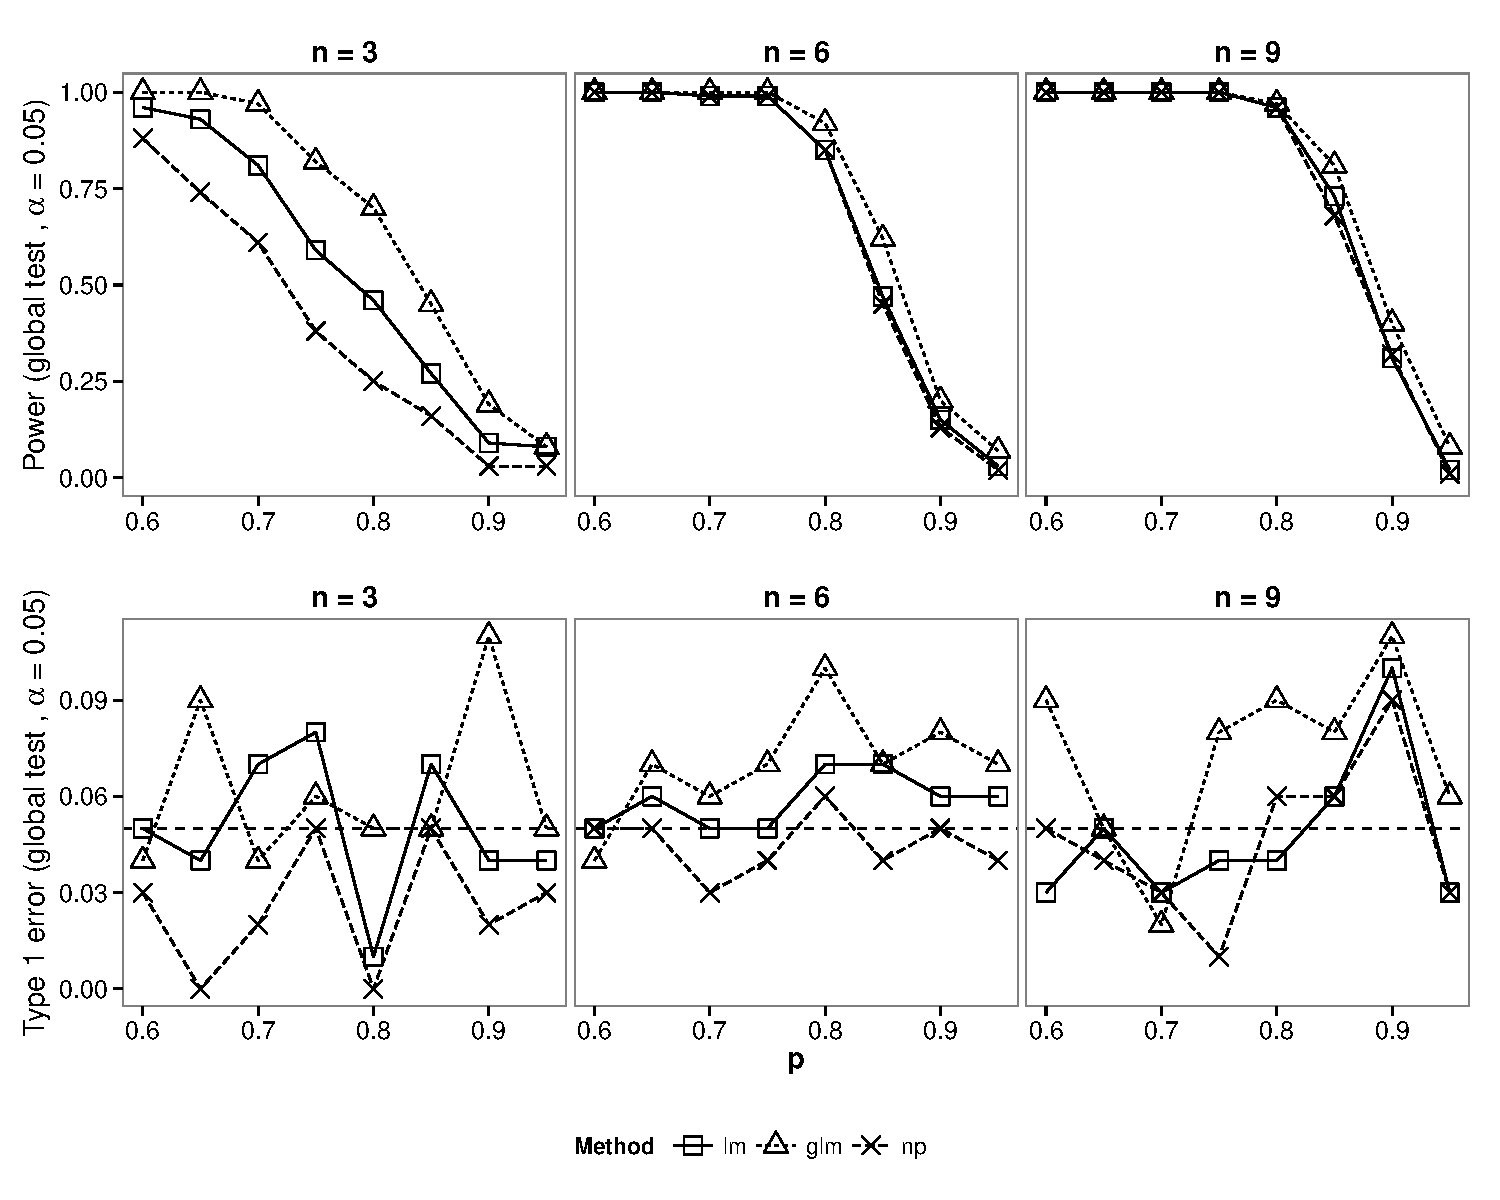
\includegraphics[width = 126mm]{p_glob_p.pdf}
  \caption{
  Binomial data simulations: 
  Type \DIFdelbeginFL \DIFdelFL{1 }\DIFdelendFL \DIFaddbeginFL \DIFaddFL{I }\DIFaddendFL error (top) and  power (bottom) for the test of a treatment effect. 
  Dashed horizontal line denotes the nominal Type \DIFdelbeginFL \DIFdelFL{1 }\DIFdelendFL \DIFaddbeginFL \DIFaddFL{I }\DIFaddendFL error rate at $\alpha = 0.05$.
  }
  \label{fig:p_glob_p}
\end{figure*}

For inference on LOEC we found that all methods were slightly conservative.
$WT$ was generally more conservative and $GLM_{bin}$ especially at low effect sizes ($p_E > 0.7$).
Inference on LOEC was not as powerful as inference on the general treatment effect.
Contrary to the general treatment effect, $LM$ showed the higher power than $GLM_{bin}$ at small sample sizes (n = {3, 6}).
$WT$ had no power for n = 3 and showed less power in the other simulation runs (Figure \ref{fig:p_loec_p}).

\begin{figure*}
  \centering
  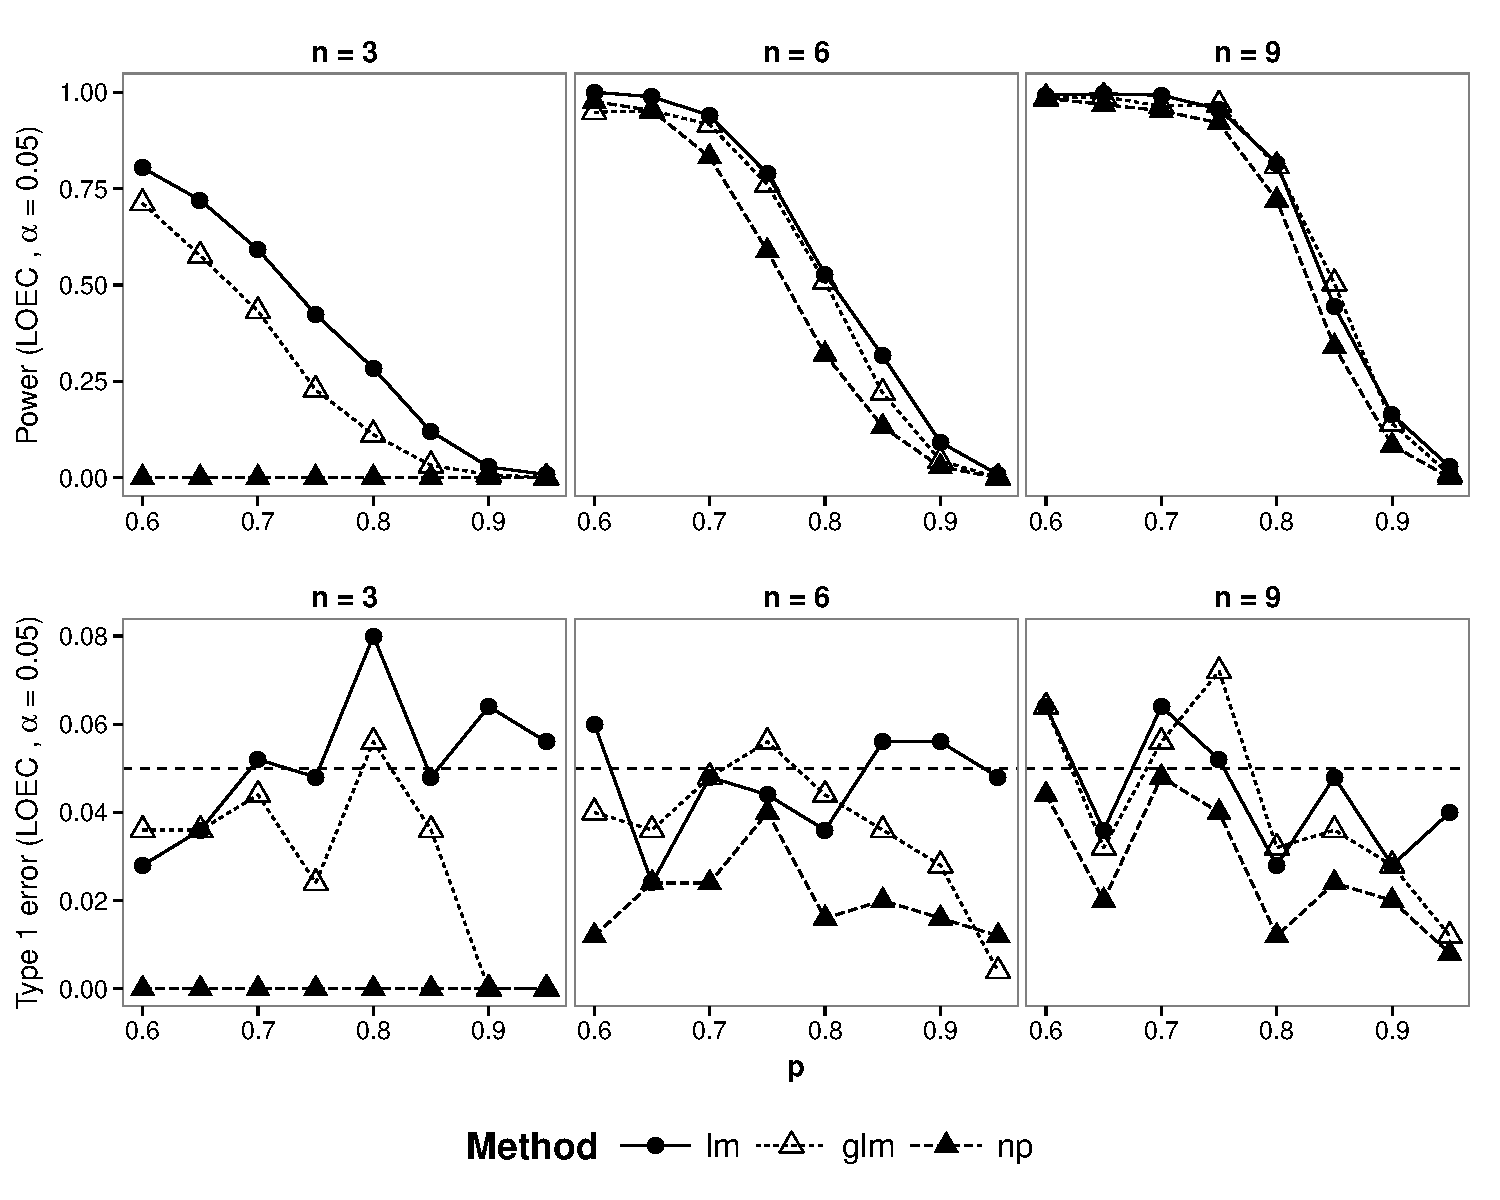
\includegraphics[width = 126mm]{p_loec_p.pdf}
  \caption{
  Binomial data simulations: 
  Type \DIFdelbeginFL \DIFdelFL{1 }\DIFdelendFL \DIFaddbeginFL \DIFaddFL{I }\DIFaddendFL error (top) and power (bottom) for the test for determination of LOEC. 
  Dashed horizontal line denotes the nominal Type \DIFdelbeginFL \DIFdelFL{1 }\DIFdelendFL \DIFaddbeginFL \DIFaddFL{I }\DIFaddendFL error rate at $\alpha = 0.05$.
  }
  \label{fig:p_loec_p}
\end{figure*}


%% ----------------------------------------------------------------------------
\section{Discussion}
\label{sec:disc}
\subsection{Case study}
%% ---- Case study
The outlined case study demonstrates that the choice of the statistical model and procedure can have substantial impact on ecotoxicological inferences and endpoints like the LOEC.
Therefore, ecotoxicologists should not base their inferences solely on statistical significance tests, but also on \DIFdelbegin \DIFdel{parameter }\DIFdelend \DIFaddbegin \DIFadd{model }\DIFaddend estimates, their uncertainty and importance \citep{gelman_difference_2006}.
Nevertheless, \citet{ohara_not_2010} showed that \DIFdelbegin \DIFdel{$LM$ using a log transformation }\DIFdelend \DIFaddbegin \DIFadd{the linear model on log transformed data }\DIFaddend gave unreliable and biased \DIFdelbegin \DIFdel{parameter }\DIFdelend estimates, whereas GLMs performed well with little bias.
Bias occurs also when back-transforming means to the original scale, which explains the lower predicted means by $LM$ in Figure \ref{fig:example} \citep{rothery_cautionary_1988} and should be corrected for \citep{newman_regression_1993}.
\DIFaddbegin \DIFadd{In fact, the linear model would results in identical treatment means as the GLMs when applied to untransformed data. 
However, predictions will differ with a continuous predictor.
}\DIFaddend 

This is further highlighted by the fact that for the same model (linear model \DIFdelbegin \DIFdel{of }\DIFdelend \DIFaddbegin \DIFadd{applied to }\DIFaddend transformed data), \citet{brock_minimum_2015} reported a 10-fold lower LOEC (\mbox{0.3 mg/L}) then found in our study (3 mg/L, Figure \ref{fig:example}).
The reasons are manifold: 
\DIFdelbegin %DIFDELCMD < \citep{brock_minimum_2015} %%%
\DIFdelend \DIFaddbegin \DIFadd{(i)~}\citet{brock_minimum_2015} \DIFaddend used a $log(2~y + 1)$ transformation, whereas we used a $log(A~y + 1)$ transformation, where A = 2 / 11 = 0.182 \citep{van_den_brink_impact_2000}.
\DIFdelbegin \DIFdel{However, this contributed only little to the differences.
A much bigger impact had the type of multiple comparison: }\DIFdelend \DIFaddbegin \DIFadd{(ii)~We adjusted for multiple testing using Holm's (}\citeyear{holm_simple_1979}\DIFadd{) method.
(iii)~}\DIFaddend \citet{brock_minimum_2015} used a one-sided Williams test \citep{williams_comparison_1972}, whereas we used one-sided comparisons to the control (Dunnett contrasts).
\DIFdelbegin \DIFdel{In contrast to the Williams test, Dunnett contrasts do not assume a monotonic dose-response relationship and allow individual comparisons between treatment groups and the control.
However, under monotonicity they have less power, }\DIFdelend \DIFaddbegin \DIFadd{The choice of transformation contributed only little to the differences. 
If the assumptions of Williams test  are met it has strictly greater power than Dunnett contrasts }\citep{jaki_statistical_2013}\DIFadd{, }\DIFaddend which explains the differences \DIFdelbegin %DIFDELCMD < \citep{jaki_statistical_2013}%%%
\DIFdel{.
Both types of multiple comparisons are available }\DIFdelend \DIFaddbegin \DIFadd{in the case study.
A generalisation of the Williams test }\DIFaddend as multiple contrast \DIFdelbegin \DIFdel{tests }\DIFdelend \DIFaddbegin \DIFadd{test (MCT) can be used }\DIFaddend in a GLM framework \DIFaddbegin \citep{hothorn_simultaneous_2008}\DIFadd{.
Nevertheless, such a Williams-type MCT is not a panacea }\citep{hothorn_statistical_2014} \DIFadd{and our simulated semi-concave dose-response relationship is a situation where it fails and likely underestimates the LOEC }\citep{kuiper_identification_2014}\DIFaddend . 
 \DIFdelbegin \DIFdel{Therefore, our comparison of methods should be independent from the choice of contrast, which is determined by assumptions and research questions. 
 }\DIFdelend 


%% ---- Guide GLMs
Overdispersion is common for ecological datasets \citep{warton_many_2005} and the case study illustrates the potential effects of overdispersion that is not accounted for: standard errors will be underestimated and significance overestimated (Figures \ref{fig:example}).
This is also shown by our simulations (Figures \ref{fig:p_glob_c}, \ref{fig:p_loec_c}) where $GLM_p$ showed increased \DIFdelbegin \DIFdel{type 1 }\DIFdelend \DIFaddbegin \DIFadd{Type I }\DIFaddend error rates because of overdispersed simulated data. 
However, in factorial designs the mean-variance relationship can be easily checked by plotting mean versus variance of the treatment groups \DIFaddbegin \DIFadd{or by inspecting residual vs. fitted values plots }\DIFaddend (see Supplement 2).
\DIFaddbegin \DIFadd{Our simulations revealed that the LR test for $GLM_{nb}$ is invalid because of increased Type I errors. This explains why it had the lowest p-value in the case study.
}

\DIFaddend In the introduction we pointed out that there is little advice how to choose between the plenty of possible transformations - how do GLMs simplify this problem?
The distribution modelled can be chosen using knowledge about the data (e.g. bounds, integer or continuous data etc).
Knowing what type of data is modelled (see Methods section), the model selection process can be completely guided by the data and diagnostic tools. Therefore, choosing an appropriate model is easier than choosing between possible transformations.


\subsection{Simulations}
%% --- general low power
Our simulations showed that \DIFdelbegin \DIFdel{generally GLMs have }\DIFdelend \DIFaddbegin \DIFadd{GLMs have generally }\DIFaddend greater power than \DIFdelbegin \DIFdel{data transformations}\DIFdelend \DIFaddbegin \DIFadd{the linear model applied to transformed data}\DIFaddend .
However, the simulations also suggest that the power at the population level in common mesocosm experiments is low.
For common samples sizes ($n \le 4$ ) and a reduction in abundance of 50\% we found a low power to detect any treatment-related effect (\textless 50\% for methods with appropriate Type \DIFdelbegin \DIFdel{1 }\DIFdelend \DIFaddbegin \DIFadd{I }\DIFaddend error, Figure \ref{fig:p_glob_c}).
Statistical power to detect the correct LOEC was even lower (less than 25\%), which can be attributed to multiple testing.
The low power of all methods to detect significant treatment levels such as the LOEC or NOEC suggests that these endpoints from ecotoxicological studies should be interpreted with caution and underpins their criticism \citep{laskowski_good_1995,landis_well_2011}.

%% --- Multivariate + GLMM -------
Mesocosm studies allow also inferences on community level. 
For community analyses \emph{GLM for multivariate data} \citep{warton_distance-based_2012} have been proposed as alternative to Principal Response Curves (PRC) and yielded \DIFdelbegin \DIFdel{to }\DIFdelend similar inferences, but better indication of responsive taxa \citep{szocs_analysing_2015}. 
However, \citet{ter_braak_topics_2014} argue to use data transformations with community data because of their simplicity and robustness.
Although our simulations covered only simple experimental designs at the population level, findings may also extend to more complex situations. 
Nested or repeated designs with non-normal data could be analysed using Generalised Linear Mixed Models (GLMM) and may have advantages with respect to power \citep{stroup_rethinking_2014}.

%% --- Alternatives -------
To counteract the problems with low power at the population level \citet{brock_minimum_2015} proposed to take the Minimum Detectable Difference (MDD), a method to assess statistical power \emph{a posteriori}, for inference into account.
However, \emph{a priori} power analyses can be performed easily using simulations, even for complex experimental designs \DIFdelbegin %DIFDELCMD < \citep{johnson_power_2014}%%%
\DIFdelend \DIFaddbegin \citep{johnson_power_2015}\DIFaddend , and might help to design, interpret and evaluate ecotoxicological studies.
Moreover, \citet{brock_minimum_2015} proposed that statistical power of mesocosm experiments can be increased by reducing sampling variability through improved sampling techniques and quantification methods, though they also caution against depleting populations through more exhaustive sampling.
As we showed, using \DIFdelbegin \DIFdel{appropriate statistical methods (like GLMs ) }\DIFdelend \DIFaddbegin \DIFadd{GLMs }\DIFaddend can enhance the power at no extra costs.

%% --- Non-parametric
\citet{wang_making_2011} advocated that in the typical case of small sample sizes (n \textless 20) and non-normal data, non-parametric tests perform better than parametric tests assuming normality.
In contrast, our results showed that the often applied $KW$ and $WT$ have less power compared to $LM$.
Moreover, $GLMs$ always performed better than non-parametric tests. 
Though more powerful non-parametric tests may be available \citep{konietschke_rank-based_2012}, these are focused on hypothesis testing and do not provide estimation of effect sizes.
Additionally to testing, GLMs allow the estimation and interpretation of effects that might not be statistically significant, but ecologically relevant.
Therefore, we advise using GLMs instead of non-parametric tests for non-normal data.

%% ---- Problems GLM
We found an increased Type-I error for $GLM_{nb}$ at low sample sizes.
However, it is well known that the LR statistic is not reliable at small sample sizes \citep{bolker_generalized_2009,wilks_large-sample_1938}.
Parametric bootstrap ($GLM_{npb}$) is a valuable alternative in such situations and maintains appropriate levels (Figure \ref{fig:p_glob_c}).
Moreover, at small sample sizes and low abundances a significant amount of negative binomial models did not converge.
We used an iterative algorithm to fit these models \citep{venables_modern_2002} and other methods assessing the likelihood directly may perform better.

$GLM_{qp}$ showed higher statistical power than $GLM_{npb}$ (Figure \ref{fig:p_glob_c}, bottom).
This could be explained by the simpler mean-variance relationship of $GLM_{qp}$ (eqn. \ref{eqn:quasi} and \ref{eqn:negbin}), because at small samples sizes, low abundances or few treatment groups it is difficult to determine the mean-variance relationship\DIFaddbegin \DIFadd{.
Our results are similar to }\citet{ives_for_2015}\DIFadd{, who compared GLMs to LM applied to transformed data for testing regression coefficients.
Because of inflated Type I errors of $GLM_{nb}$ and , in the case of multiple regression, inflated Type I errors of $GLM_{qp}$ he concluded that the approach of transforming data and applying LMs provides a robust method and should be preferred.
We showed that the parametric bootstrap LR test of $GLM_{nb}$ provides appropriate Type I errors and bootstrapping might be also an alternative for testing coefficients.
However, bootstrapping is computationally very intensive and we found no gains in power compared to $GLM_{qp}$ (Figure \ref{fig:p_glob_c}). 
Because of higher power, appropriate Type I errors, stable convergence and reduced bias }\citep{ohara_not_2010} \DIFadd{we conclude that count data in one factorial experiments should be analysed using the quasi-Poisson model}\DIFaddend .

%% --- binomial data
Binomial data are often collected in lab trials, where increasing the sample size may be relatively easy to accomplish. 
We found notable differences in power to detect a treatment effect for all simulated sample sizes.
Similarly, \citet{warton_arcsine_2011} also found that GLMs have higher power than arcsine transformed linear models.
Though we did not simulate overdispersed binomial data, this should be checked and accounted for.
In such situations a GLMM may offer an appealing alternative \citep{warton_arcsine_2011}.
At low effect sizes $GLM_{bin}$ became conservative with increasing $\pi_C$, although this effect lessened as sample size increased (Figure \ref{fig:p_loec_p}). 
This is because $\pi$ approaches its boundary and is also known as the \emph{Hauck-Donner effect} \citep{hauck_walds_1977}. A LR-Test or parametric bootstrap may provide an alternative in such situations \citep{bolker_generalized_2009}.
This can also explain why $LM$ performed better for deriving LOECs at low sample sizes.

GLMs can be fitted with several statistical software packages and many textbooks are available to introduce ecotoxicologists to these models (e.g. \citealt{zuur_beginners_2013} or \citealt{quinn_experimental_2009}).
We recommend that ecotoxicologists should change their models instead of their data.
GLMs should become a standard method in ecotoxicology and incorporated into respective guidelines.


\section{Compliance with Ethical Standards}
Conflict of Interest: The authors declare that they have no conflict of interest.

%% --------------------------------
\bibliography{references}
\bibliographystyle{spbasic}

\end{document}
